% tmfem technical report. Build:  cd report && latexmk -pdf main.tex
% Every computed number is a macro from generated/numbers.tex (scripts/report_numbers.py); sources are
% listed in docs/PROVENANCE.md. Literal numbers in this file are inputs (case files, material data) or
% values of docs/REFERENCE_VALUES.md, recomputed by references/verify_reference_values.py.
\documentclass[11pt,a4paper]{article}
\usepackage[margin=2.0cm]{geometry}
\usepackage[T1]{fontenc}
\usepackage{lmodern}
\usepackage{microtype}
\usepackage{amsmath,amssymb}
\usepackage{graphicx}
\usepackage{booktabs}
\usepackage{subcaption}
\usepackage[detect-all]{siunitx}
\usepackage[numbers,sort&compress]{natbib}
\usepackage{xcolor}
\usepackage[colorlinks=true,linkcolor=blue!50!black,citecolor=blue!50!black,urlcolor=blue!50!black]{hyperref}
\usepackage[nameinlink,capitalise]{cleveref}

\graphicspath{{../docs/figures/}}
\sisetup{exponent-product=\times, retain-explicit-plus=true}
% Generated by scripts/report_numbers.py from the run at commit 8d914ab. Do not edit.
% Sources: docs/PROVENANCE.md
\newcommand{\NPbTimeFE}{\num{25373.7}}
\newcommand{\NPbTimeRef}{\num{25370.2}}
\newcommand{\NPhDrift}{\num{3.7e-12}}
\newcommand{\NPhSlope}{\num{-0.499996}}
\newcommand{\NPiBiot}{\num{0.00183}}
\newcommand{\NPiTau}{\num{549.5}}
\newcommand{\NPjDiff}{\num{0.033}}
\newcommand{\NPkDiff}{\num{0.0256}}
\newcommand{\NPmBE}{\num{0.98}}
\newcommand{\NPmCN}{\num{2.00}}
\newcommand{\NPmBEf}{\num{1.00}}
\newcommand{\NPmCNf}{\num{2.00}}
\newcommand{\NPmSpace}{\num{2.00}}
\newcommand{\NPmSpaceLumped}{\num{2.01}}
\newcommand{\NPaPatchTthree}{\num{5.8e-15}}
\newcommand{\NPaPatchTsix}{\num{8e-14}}
\newcommand{\NKtTsix}{\num{2.99969}}
\newcommand{\NKtTthree}{\num{2.973}}
\newcommand{\NPdErr}{\num{0.0044}}
\newcommand{\NPeErr}{\num{0.012}}
\newcommand{\NPfTthreeLtwo}{\num{1.97}}
\newcommand{\NPfTthreeEn}{\num{0.99}}
\newcommand{\NPfTsixLtwo}{\num{3.11}}
\newcommand{\NPfTsixEn}{\num{1.97}}
\newcommand{\NPfTsixLtwoPe}{\num{3.12}}
\newcommand{\NFitSy}{\num{309.1}}
\newcommand{\NFitK}{\num{520.9}}
\newcommand{\NFitM}{\num{0.362}}
\newcommand{\NFitS}{\num{4.58}}
\newcommand{\NLogLogM}{\num{0.385}}
\newcommand{\NLogLogK}{\num{548}}
\newcommand{\NPbEyy}{\num{0.031581}}
\newcommand{\NPbExx}{\num{-0.01535}}
\newcommand{\NPcZ}{\num{1.59}}
\newcommand{\NPdRatePe}{\num{2.12}}
\newcommand{\NPdRatePs}{\num{2.62}}
\newcommand{\NPeBar}{\num{1.1e-12}}
\newcommand{\NPsEpsFE}{\num{0.002356}}
\newcommand{\NPsAlphaFE}{\num{0.000815}}
\newcommand{\NPsSigFE}{\num{318.7}}
\newcommand{\NPsZone}{\num{0.174}}
\newcommand{\NPsSyyMax}{\num{331.2}}
\newcommand{\NPeZone}{\num{0.0749}}
\newcommand{\NPeSyyEdge}{\num{357.9}}
\newcommand{\NDiskSrZero}{\num{-0.24996}}
\newcommand{\NDiskSrHalf}{\num{-0.18748}}
\newcommand{\NDiskSrOne}{\num{2.2e-05}}
\newcommand{\NDiskStZero}{\num{-0.24996}}
\newcommand{\NDiskStHalf}{\num{-0.062477}}
\newcommand{\NDiskStOne}{\num{0.500014}}
\newcommand{\NGaussVarTthree}{\num{0.00035}}
\newcommand{\NGaussVarTsix}{\num{7.8e-09}}
\newcommand{\NGaussEnTsix}{\num{5.8e-14}}
\newcommand{\NPgTthreeLtwo}{\num{2.02}}
\newcommand{\NPgTthreeEn}{\num{1.01}}
\newcommand{\NPgTsixLtwo}{\num{3.06}}
\newcommand{\NPgTsixEn}{\num{2.04}}
\newcommand{\NPhTthree}{\num{1.95}}
\newcommand{\NPhTsix}{\num{3.08}}
\newcommand{\NNeuberEps}{\num{0.002647}}
\newcommand{\NNeuberAlpha}{\num{0.001098}}
\newcommand{\NNeuberSig}{\num{321.3}}
\newcommand{\NPsEpsDiff}{\num{-11.0}\,\%}
\newcommand{\NPsAlphaDiff}{\num{-25.7}\,\%}
\newcommand{\NPsSigDiff}{\num{-0.8}\,\%}
\newcommand{\NPfPlaneDiff}{\num{0.012}}
\newcommand{\NRows}{\num{115}}
\newcommand{\NAsserted}{\num{89}}
\newcommand{\NIds}{\num{32}}
\newcommand{\NWorstUse}{\num{80}\,\%}
\newcommand{\NFitDof}{\num{5}}
\newcommand{\NBandMax}{\num{2.24}}
\newcommand{\NPjDiffHalf}{\num{0.026}}
\newcommand{\NTests}{\num{93}}
\newcommand{\NFailed}{\num{0}}
\newcommand{\NSkipped}{\num{1}}
\newcommand{\NPeSzz}{\num{124}}
\newcommand{\NPhTimePartTthree}{\num{2}\,\%}
\newcommand{\NPhTimePartTsix}{\num{50}\,\%}
\newcommand{\NPfLoadIdentity}{\num{5.5e-17}}
\newcommand{\NPsZoneLevelOne}{\num{0.159}}
\newcommand{\NDemoCuHalfdT}{\num{184}}
\newcommand{\NDemoCuHalfvm}{\num{296}}
\newcommand{\NDemoCuHalfTmax}{\num{477}}
\newcommand{\NDemoCuHalfratio}{\num{4.29}}
\newcommand{\NDemoCuHalfgps}{\num{0.064}\,\%}
\newcommand{\NDemoCuOnedT}{\num{46.2}}
\newcommand{\NDemoCuOnevm}{\num{74.3}}
\newcommand{\NDemoCuOneTmax}{\num{339}}
\newcommand{\NDemoCuOneratio}{\num{1.08}}
\newcommand{\NDemoCuOnegps}{\num{0.26}\,\%}
\newcommand{\NDemoCuTwodT}{\num{11.6}}
\newcommand{\NDemoCuTwovm}{\num{18.7}}
\newcommand{\NDemoCuTwoTmax}{\num{305}}
\newcommand{\NDemoCuTworatio}{\num{0.271}}
\newcommand{\NDemoCuTwogps}{\num{1}\,\%}
\newcommand{\NDemoCuFourdT}{\num{2.89}}
\newcommand{\NDemoCuFourvm}{\num{4.7}}
\newcommand{\NDemoCuFourTmax}{\num{296}}
\newcommand{\NDemoCuFourratio}{\num{0.0688}}
\newcommand{\NDemoCuFourgps}{\num{4.1}\,\%}
\newcommand{\NDemoGrHalfdT}{\num{489}}
\newcommand{\NDemoGrHalfvm}{\num{14.8}}
\newcommand{\NDemoGrHalfTmax}{\num{782}}
\newcommand{\NDemoGrHalfratio}{\num{0.054}}
\newcommand{\NDemoGrHalfgps}{\num{0.079}\,\%}
\newcommand{\NDemoGrHalfcomp}{\num{0.23}}
\newcommand{\NDemoGrOnedT}{\num{123}}
\newcommand{\NDemoGrOnevm}{\num{3.7}}
\newcommand{\NDemoGrOneTmax}{\num{416}}
\newcommand{\NDemoGrOneratio}{\num{0.0138}}
\newcommand{\NDemoGrOnegps}{\num{0.31}\,\%}
\newcommand{\NDemoGrOnecomp}{\num{0.057}}
\newcommand{\NDemoGrTwodT}{\num{30.7}}
\newcommand{\NDemoGrTwovm}{\num{0.94}}
\newcommand{\NDemoGrTwoTmax}{\num{324}}
\newcommand{\NDemoGrTworatio}{\num{0.00366}}
\newcommand{\NDemoGrTwogps}{\num{1.3}\,\%}
\newcommand{\NDemoGrTwocomp}{\num{0.014}}
\newcommand{\NDemoGrFourdT}{\num{7.67}}
\newcommand{\NDemoGrFourvm}{\num{0.24}}
\newcommand{\NDemoGrFourTmax}{\num{301}}
\newcommand{\NDemoGrFourratio}{\num{0.00115}}
\newcommand{\NDemoGrFourgps}{\num{5}\,\%}
\newcommand{\NDemoGrFourcomp}{\num{0.0035}}
\newcommand{\NDemoGapdT}{\num{0.5}\,\%}
\newcommand{\NDemoGapvm}{\num{4.4}\,\%}
\newcommand{\NHeatRatio}{\num{2.65}}
\newcommand{\NFomCu}{\num{0.93}}
\newcommand{\NFomGr}{\num{0.047}}
\newcommand{\NStressRatio}{\num{20}}
\newcommand{\NCuYield}{\num{69}}
\newcommand{\NRelaxTenms}{\num{31}\,\%}
\newcommand{\NRelaxHundredms}{\num{4.4}\,\%}
\newcommand{\NJanafT}{\num{612}}
\newcommand{\NJanafdT}{\num{319}}
\newcommand{\NConstdT}{\num{491}}
\newcommand{\NJanafOver}{\num{54}\,\%}
\newcommand{\NCpRatio}{\num{2.3}}


\newcommand{\tmfem}{\texttt{tmfem}}
\newcommand{\vect}[1]{\boldsymbol{#1}}
\newcommand{\refrow}[1]{\textsf{#1}}

\title{\tmfem: a validated two-dimensional thermo-mechanical\\finite-element solver written from scratch}
\author{TODO: name, affiliation}
\date{\today}

\begin{document}
\maketitle

\begin{abstract}
\noindent \tmfem{} is a C++17 finite-element solver for 1D and 2D transient heat conduction and diffusion,
2D linear elasticity, small-strain von Mises elastoplasticity and one-way thermo-mechanical coupling.
It uses no FEM library. Every capability is tied to a validation test against an analytical
solution, a recomputed textbook result or a reference simulation, with an explicit tolerance. The suite has \NTests{} tests: \NFailed{} fail, and \NSkipped{} is skipped (see below). They record \NRows{} values for \NIds{}
reference rows; one more reference row (an ANSYS comparison) is skipped because its data were never
provided. Observed orders of convergence match theory on four mesh levels: the T6 Kirsch plate converges
at order \NPfTsixLtwo{} in the $L^2$ norm and \NPfTsixEn{} in the energy norm (levels 1--4, see \cref{sec:corrections}), and it gives a stress
concentration factor of \NKtTsix{} (exact: 3). A beam-heated block, explicitly a demonstration
rather than a validation, illustrates the workflow used for beam-intercepting devices: at equal
deposited energy, graphite has a \NHeatRatio{} times larger temperature rise than copper yet carries
\NStressRatio{} times less stress. \tmfem{} is a learning and verification project. It does not replace ANSYS or Abaqus.
\end{abstract}

% ---------------------------------------------------------------------------------------------------
\section{Context and goals}\label{sec:context}

Beam-intercepting devices at CERN (targets, collimators, absorbers, dumps) are designed in two steps. A
Monte Carlo transport code such as FLUKA~\cite{fluka2005} or Geant4~\cite{geant4} computes where the
beam deposits its energy. A finite-element code (in practice ANSYS) then computes the temperature
field and the thermal stresses it causes, and these are checked against the strength of the material.
\tmfem{} rebuilds the second step from first principles, at small scale, as a way to understand
and verify each ingredient: the weak forms, the element technology, time integration, return mapping
plasticity and the thermal load.

The guiding rule is that no capability is claimed without a test that proves it. Each benchmark
has a reference value and a tolerance in a reference table. Most rows were written before the code;
the rows for 2D heat with source and convection and for the phase-4 convergence orders (P4-f to P4-h)
were written in phase 4 together with their tests, as were the plane-strain targets of P4-a and P4-b. Every
convergence claim is backed by an observed order measured on at least three refinements. The source
material for the benchmarks (lab exercises by M.~R.~Kabiri, ENSAM Mekn\`es~\cite{kabiri_labs})
contains several wrong values. Each reference was therefore recomputed by a script, and the
disagreements are listed in \cref{sec:corrections}. A test was never tuned to match a reference. When a
result missed its tolerance, the cause was found, and any change to the test plan was approved and is
disclosed (\cref{sec:corrections}).

\paragraph{Scope.} In scope: 1D and 2D transient heat and diffusion; 2D linear elasticity in plane stress
and plane strain; small-strain J2 plasticity with isotropic hardening; one-way thermal-to-mechanical
coupling; VTU output for ParaView. Out of scope: 3D, large deformation, dynamics and stress waves,
temperature-dependent properties, contact, radiation and real particle-shower energy maps.

% ---------------------------------------------------------------------------------------------------
\section{Methods}\label{sec:methods}

\subsection{Heat conduction and diffusion}
The heat equation $\rho c\,\dot T = \nabla\cdot(k\nabla T) + q$ is discretised with standard Galerkin
finite elements. Boundary conditions are Dirichlet, prescribed flux, or convective
$-k\,\partial T/\partial n = h\,(T - T_\infty(t))$, with $T_\infty(t)$ read from a time series and
interpolated linearly. Diffusion uses the same code with $\rho c = 1$ and $k = D$. With capacity matrix
$\vect M$ (consistent, or row-sum lumped in 1D), conductivity-plus-Robin matrix $\vect A$ and load
$\vect F$, the $\theta$-method reads
\begin{equation}
  (\vect M + \theta\,\Delta t\,\vect A)\,\vect T^{n+1}
  = (\vect M - (1-\theta)\,\Delta t\,\vect A)\,\vect T^{n}
  + \Delta t\,\big[\theta\,\vect F^{n+1} + (1-\theta)\,\vect F^{n}\big],
  \label{eq:theta}
\end{equation}
with $\theta = 1$ (backward Euler, BE) or $\theta = 1/2$ (Crank--Nicolson, CN). Backward Euler is used
when $\Delta t$ is much larger than the diffusion time of an element. Crank--Nicolson is not
L-stable and makes the stiff modes ring there~\cite{thomee}. Dirichlet values are imposed by
elimination. The same integrator serves 1D (linear elements) and 2D (T3 and T6 triangles,
volumetric source, convective edges and a convective face sink for thin plates).

\subsection{Linear elasticity}
Displacements are interpolated with three-node (T3) or six-node (T6) isoparametric triangles. On a
curved boundary the T6 mid-side nodes lie on the curve. Gmsh~\cite{gmsh} places them there, and this
is required for optimal convergence on the hole of the Kirsch plate~\cite{strang_fix}. The
stiffness is $\vect K = \sum_e\int_{\Omega_e}\vect B^{T}\vect D\,\vect B\,\mathrm{d}A$ in Voigt order
$[xx, yy, xy]$ with engineering shear strain, and $\vect D$ is the plane-stress or plane-strain
elasticity matrix. Quadrature uses one point for T3 and three for T6 stiffness. Nonlinear residuals use one point (T3) or
the six-point degree-4 rule~\cite{dunavant1985} (T6), and error norms collapsed Gauss rules (16 points for elasticity, 25 for heat). Tractions are
integrated along element edges. Stresses are evaluated at quadrature points, or at any point inside
the element that contains it (averaged over elements that share the point). Nodal averages are used
only for plots and VTU output. Meshes are read from Gmsh 4.1 ASCII files, which the build generates
from committed \texttt{.geo} files with Gmsh pinned to version 4.12.1, so that the same Gmsh build gives
the same meshes everywhere.

\subsection{Elastoplasticity}
The material model is small-strain J2 plasticity with isotropic hardening $\sigma_y(\alpha)$, where
$\alpha$ is the accumulated equivalent plastic strain. It is integrated by the backward-Euler radial
return~\cite{simo_hughes,desouzaneto}. Given the trial deviatoric stress $\vect s^{tr}$ and
$q^{tr} = \sqrt{3/2}\,\lVert\vect s^{tr}\rVert$, the plastic multiplier solves the scalar equation
$q^{tr} - 3G\,\Delta\gamma - \sigma_y(\alpha_n + \Delta\gamma) = 0$ by Newton's method. The consistent
(algorithmic) tangent~\cite{simo_taylor1985} is
\begin{equation}
  \vect C^{alg} = \kappa\,\vect 1\otimes\vect 1
  + 2G\Big(1 - \frac{3G\Delta\gamma}{q^{tr}}\Big)\mathbb I_{dev}
  + 6G^2\Big(\frac{\Delta\gamma}{q^{tr}} - \frac{1}{3G + H}\Big)\,\bar{\vect n}\otimes\bar{\vect n},
  \qquad \bar{\vect n} = \frac{\vect s^{tr}}{\lVert\vect s^{tr}\rVert},
  \label{eq:calg}
\end{equation}
where $\kappa$ is the bulk modulus and $H = \mathrm d\sigma_y/\mathrm d\alpha$. Two hardening laws sit
behind one interface. The first is a piecewise-linear table built from the true tensile curve, with
$\alpha = \varepsilon - \sigma/E$. The second is Ludwik's law~\cite{ludwik1909}
$\sigma_y = \sigma_{y0} + K\alpha^{m}$, fitted to the same data by least squares, with a covariance
estimate and a leave-one-out jackknife for the uncertainty. Plane strain runs the 3D algorithm exactly
on the four components $[xx, yy, zz, xy]$. In plane stress each quadrature point solves for
$\varepsilon_{zz}$ by a local Newton iteration so that $\sigma_{zz} = 0$. The tangent is then condensed,
$D_{\alpha\beta} = C_{\alpha\beta} - C_{\alpha z}C_{z\beta}/C_{zz}$. The global equations are solved by
Newton--Raphson with load stepping, and history variables are updated only from the converged state of
the previous step. A material-point driver iterates the lateral strains until the lateral stresses
vanish; this reproduces the uniaxial tensile test.

\subsection{Thermo-mechanical coupling}
The temperature field from the heat solver, on the same mesh, enters the mechanical problem as an
eigenstrain $\alpha_{th}(T - T_{ref})$. Writing $\vect m = [1, 1, 0]^T$, the thermal load vector is
\begin{equation}
  \vect f_{th} = \sum_e\int_{\Omega_e}\vect B^{T}\vect m\,\beta\,\Delta T_h\,\mathrm dA,\qquad
  \beta = \frac{E\alpha_{th}}{1-\nu}\ \text{(plane stress)},\quad
  \beta = \frac{E\alpha_{th}}{1-2\nu}\ \text{(plane strain)},
\end{equation}
and stress recovery subtracts $\beta\,\Delta T_h\,\vect m$. In plane strain the out-of-plane stress is
$\sigma_{zz} = \nu(\sigma_{xx} + \sigma_{yy}) - E\alpha_{th}\Delta T$. The case output once dropped the
thermal term here, until an output test caught it. The coupling is one way and quasi-static: stress
does not feed back into the temperature, and inertia is neglected.

\subsection{Software and verification set-up}
The code is about forty small C++17 translation units in \texttt{mesh}, \texttt{fem},
\texttt{thermal}, \texttt{mechanics}, \texttt{coupling} and \texttt{io}. It depends only on the standard
library, Eigen~3~\cite{eigen} (sparse Cholesky $LDL^T$ for symmetric systems, sparse LU otherwise),
nlohmann/json for case files and Catch2 for tests. Cases are small JSON files. Each validation test
writes the value it asserts to a CSV file next to its reference and tolerance. The README results table
and \cref{tab:results} are generated from these files. Every other computed number in this report is
generated from test or solver output by a script that also writes its source
(\texttt{docs/PROVENANCE.md}). Inputs and reference values are quoted from the case files and
\texttt{docs/REFERENCE\_VALUES.md}. Continuous integration builds the code with warnings as errors and
runs every test except the two slow elastoplastic plate tests on every push. The full suite is a
manually started workflow.

% ---------------------------------------------------------------------------------------------------
\section{Validation}\label{sec:validation}

\Cref{tab:results} summarises the suite. For each reference row it shows the recorded quantity that
uses the largest share of its tolerance; the README lists all \NRows{} values with their test names.
The worst two-sided row uses \NWorstUse{} of its tolerance; the one-sided Newton-rate row (P3-d, scored as
threshold over value) is at \NOneSidedUse{}. The 2D orders (P2-f, P4-g, P4-h) are least-squares slopes of
$\log e$ against $\log h$ over levels 1--4; level 0 is computed and printed but excluded from the fit
(see \cref{sec:corrections}). The 1D orders (P1-m) use all four levels.

\begin{table}[tbp]
  \centering\scriptsize\renewcommand{\arraystretch}{0.9}
  % Generated by scripts/report_numbers.py from the run at commit a6944f8. Do not edit.
\begin{tabular}{@{}l p{2.8cm} p{4.1cm} r r p{1.8cm} r@{}}
\toprule
ID & Benchmark & Quantity (largest use of tolerance) & Reference & tmfem & Tolerance & Use \\
\midrule
P1-a & Steady diffusion flux (ex. 1) & J finite element & \num{2.4e-09} & \num{2.4e-09} & 1e-12 relative & 0\,\% \\
P1-b & Carburizing, erf solution (ex. 2) & time finite element [s] & \num{25370} & \num{25373.7} & 0.5\% & 3\,\% \\
P1-c & Equivalent time (ex. 3) & t at 500 C [h] & \num{110.4} & \num{110.417} & 0.001 relative & 15\,\% \\
P1-d & Arrhenius D(T) (ex. 4) & D(800 K) [m2/s] & \num{2.14e-15} & \num{2.1396e-15} & 0.005 relative & 4\,\% \\
P1-e & Boron predeposition dose (ex. 5) & dose formula [at/cm2] & \num{4.062e+15} & \num{4.06217e+15} & 0.005 relative & 1\,\% \\
P1-f & Thin-film surface concentration (ex. 5) & surface C at 1200 C [at/cm3] & \num{6.97e+19} & \num{6.97382e+19} & 0.005 relative & 11\,\% \\
P1-g & Arrhenius fit (ex. 5) & D(1300 C) [cm2/s] & \num{1.74e-11} & \num{1.74154e-11} & 0.005 relative & 18\,\% \\
P1-h & Thin film on a half-space & max relative dose drift & \num{0} & \num{3.69059e-12} & 1e-10 & 4\,\% \\
P1-i & Steel plate parameters & Biot number & \num{0.00183} & \num{0.00183333} & +/- 5e-6 (last quoted digit) & 67\,\% \\
P1-j & Steel plate, FE vs lumped ODE & max abs inner face FE - lumped [K] & \num{0} & \num{0.0330652} & 0.05 K & 66\,\% \\
P1-k & Steel plate, through-thickness difference & max through-thickness difference [K] & \num{0.0255348} & \num{0.0255832} & 5\% & 4\,\% \\
P1-m & 1D heat convergence orders & time order BE & \num{1} & \num{0.98331} & +/- 0.15 & 11\,\% \\
P2-a & Patch test, distorted mesh & T6 max relative error (u, sigma) & \num{0} & \num{7.96939e-14} & 1e-10 relative & 0\,\% \\
P2-b & Uniform bar in tension & T6 max rel error of end displacement & \num{0} & \num{1.22986e-13} & 1e-8 relative & 0\,\% \\
P2-c & Kirsch plate, stress concentration & Kt finest T6 & \num{3} & \num{2.99969} & 1\% & 1\,\% \\
P2-d & Kirsch plate, r/a = 2 and 4 & max abs stress error, 20 rows x 3 components [MPa] & \num{0} & \num{0.00441135} & 2 MPa & 0\,\% \\
P2-e & Kirsch plate, r/a = 1.5 & max abs stress error, 10 rows x 3 components [MPa] & \num{0} & \num{0.0117644} & 2 MPa & 1\,\% \\
P2-f & Kirsch convergence orders & T6 plane strain L2 order (levels 1-4) & \num{3} & \num{3.12065} & +/- 0.15 & 80\,\% \\
P3-a & Ludwik fit to the true tensile curve & log-log K [MPa] (sigma\_y fixed) & \num{548} & \num{547.608} & 0.5\% & 14\,\% \\
P3-b & Material point, uniaxial, tabulated hardening & eps\_yy at 457.24 MPa & \num{0.03158} & \num{0.031581} & 0.5\% & 1\,\% \\
P3-c & Material point, Ludwik along the true curve & max \textbar{}driver - data\textbar{} / s, LSQ Ludwik, 7 points & \num{0} & \num{1.5942} & +/- 2 s & 80\,\% \\
P3-d & Newton convergence rate & Newton rate, last qualifying triple, plane-strain bar, Ludwik & \num{2} & \num{2.12018} & \textgreater{}= 1.8 & 85\,\% \\
P3-e & Plane-strain bar FE vs material point & max relative difference FE vs driver (T3, T6, tabulated, Ludwik) & \num{0} & \num{1.11596e-12} & 1e-6 relative & 0\,\% \\
P3-f & Elastoplastic hole plate, S = 140 MPa (report only) & \multicolumn{5}{l}{report only (20 values), see \S\ref{sec:plasticity}} \\
P4-a & Bar held in x, uniform dT & T6 plane strain max rel error of sigma\_xx & \num{0} & \num{1.0396e-13} & 1e-8 relative & 0\,\% \\
P4-b & Free body, uniform dT & T6 plane strain max stress over beta dT & \num{0} & \num{5.26508e-14} & 1e-10 relative & 0\,\% \\
P4-c & Thin disk, parabolic T: sigma\_r & sigma\_r over E alpha dT at r/b = 0.0 & \num{-0.25} & \num{-0.249959} & 1\% & 2\,\% \\
P4-d & Thin disk, parabolic T: sigma\_theta & sigma\_theta over E alpha dT at r/b = 0.5 & \num{-0.0625} & \num{-0.0624774} & 1\% & 4\,\% \\
P4-e & 2D Gaussian heat spreading & T3 max rel variance error & \num{0} & \num{0.00034937} & 0.5\% & 7\,\% \\
P4-f & 2D heat with source and convection & (iii) amplification T6 theta 0.5 & \num{0} & \num{4.24482e-11} & 1e-10 relative & 42\,\% \\
P4-g & Thin disk convergence orders & T6 plane stress L2 order (levels 1-4) & \num{3} & \num{3.05664} & +/- 0.15 & 38\,\% \\
P4-h & 2D Gaussian heat convergence orders & T6 L2 order (levels 1-4) & \num{3} & \num{3.07825} & +/- 0.15 & 52\,\% \\
P1-l & Steel plate, real ttab vs ANSYS & \multicolumn{5}{l}{skipped: references/data/ttab.csv and the ANSYS curve are not provided} \\
\bottomrule
\end{tabular}

  \caption{Validation summary, one row per reference row of \texttt{docs/REFERENCE\_VALUES.md}. ``Use''
  is $\lvert\text{error}\rvert$ divided by the tolerance, in the tolerance's own units (threshold over value for
  the Newton rate). Generated from the test records by \texttt{scripts/report\_numbers.py}.}
  \label{tab:results}
\end{table}

\subsection{Heat conduction and diffusion}
\emph{Carburizing} (\refrow{P1-b}) is solved on a semi-infinite domain truncated at more than
$10\sqrt{Dt}$. The time for the carbon content to reach \SI{0.8}{wt\%} at \SI{0.5}{mm} is
\NPbTimeFE~\si{s}, against \NPbTimeRef~\si{s} from the error-function solution~\cite{crank}.
\emph{A thin film on a half-space} (\refrow{P1-h}), started from the analytic profile at small
$t_0 > 0$, conserves the dose to \NPhDrift{} relative, and its peak decays with slope \NPhSlope{}
(theory $-1/2$). The diffusion exercises \refrow{P1-a} to \refrow{P1-g} check closed-form results, and FE solutions where
the exercise has a field, against recomputed values.

\emph{The steel plate} (\refrow{P1-i}--\refrow{P1-k}), \SI{5}{mm} thick and convective on both faces, is
thermally thin: Biot number \NPiBiot{}, time constant \NPiTau~\si{s}. Driven by a synthetic daily
sol-air signal, the 1D FE inner-face temperature stays within \NPjDiff~\si{K} of a lumped ODE solved
with RK4 (\NPjDiffHalf~\si{K} at half the time step). The difference is partly backward-Euler time error
and partly the physical gap, of order Biot, between the face and the plate mean. The largest
through-thickness difference is \NPkDiff~\si{K}, as predicted by the quasi-steady resistance network.
The comparison with the source's ANSYS run (\refrow{P1-l}) is not done: the real input file and the
ANSYS curve were never provided.

\emph{Convergence} (\refrow{P1-m}, \cref{fig:conv}a). On four levels (three refinements) the observed temporal orders
are \NPmBE{} (BE) and \NPmCN{} (CN) on an eigenmode problem, and \NPmBEf{} and \NPmCNf{} with a source,
time-dependent Dirichlet data and Robin conditions. The spatial order is \NPmSpace{} with consistent
and \NPmSpaceLumped{} with lumped capacity.

\subsection{Linear elasticity}
\emph{Patch test} (\refrow{P2-a}): a linear displacement field is reproduced on a distorted mesh to
\NPaPatchTthree{} (T3) and \NPaPatchTsix{} (T6) relative error, and the uniform bar
(\refrow{P2-b}) to round-off.

\emph{Kirsch plate} (\refrow{P2-c}--\refrow{P2-f}). A circular hole of radius $a$ in an infinite plate
under remote stress $S = \SI{140}{MPa}$ along $y$~\cite{kirsch1898,timoshenko_goodier} is modelled as
the quarter $[0, 5a]^2$ with symmetry conditions. The exact Kirsch tractions are applied on the outer
edges, so the finite model represents the infinite plate exactly and the FE solution converges to the
analytic field. On the finest T6 mesh the stress concentration factor is \NKtTsix{} (T3: \NKtTthree{}),
and the 60 tabulated stress components at $r/a = 2$ and 4 agree within \NPdErr~\si{MPa}
(tolerance \SI{2}{MPa}), the 30 at $r/a = 1.5$ within \NPeErr~\si{MPa}. The observed orders
(\cref{fig:conv}b) are \NPfTthreeLtwo{} and \NPfTthreeEn{} for T3 ($L^2$, energy; theory 2 and 1) and
\NPfTsixLtwo{} and \NPfTsixEn{} for T6 (theory 3 and 2), in plane stress. The plane-strain orders differ from these by at most \NPfPlaneDiff{}.

\begin{figure}[tbp]
  \centering
  \begin{subfigure}{0.32\linewidth}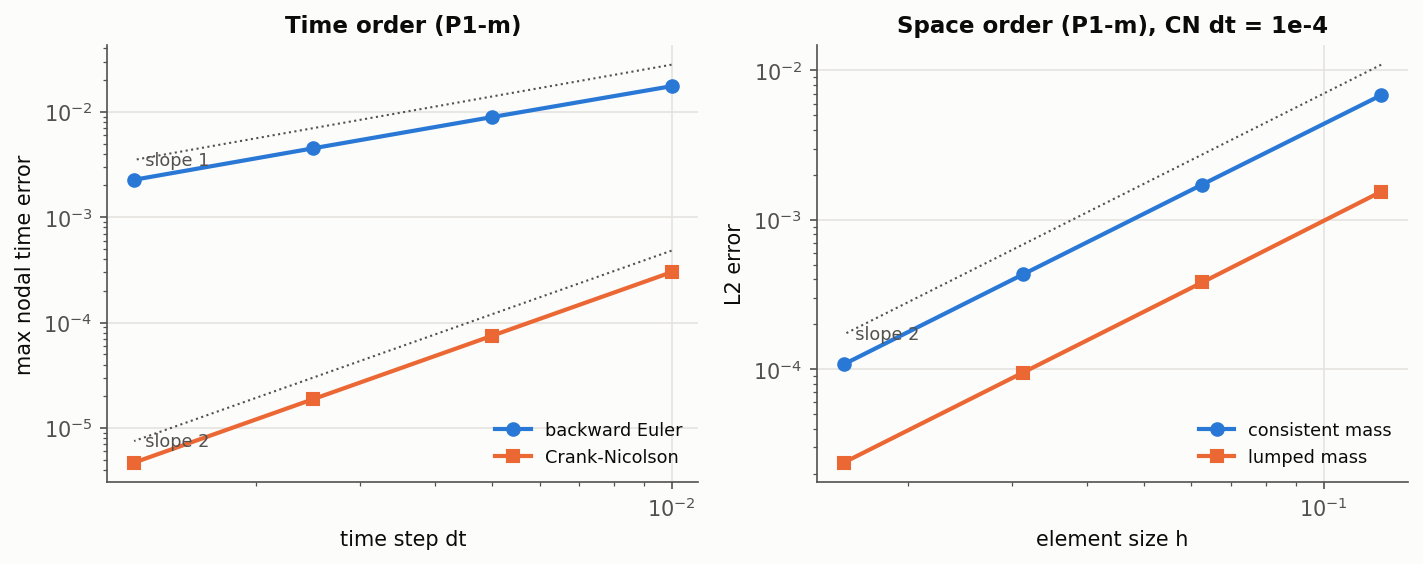
\includegraphics[width=\linewidth]{phase1_convergence}\caption{1D heat (P1-m)}\end{subfigure}\hfill
  \begin{subfigure}{0.32\linewidth}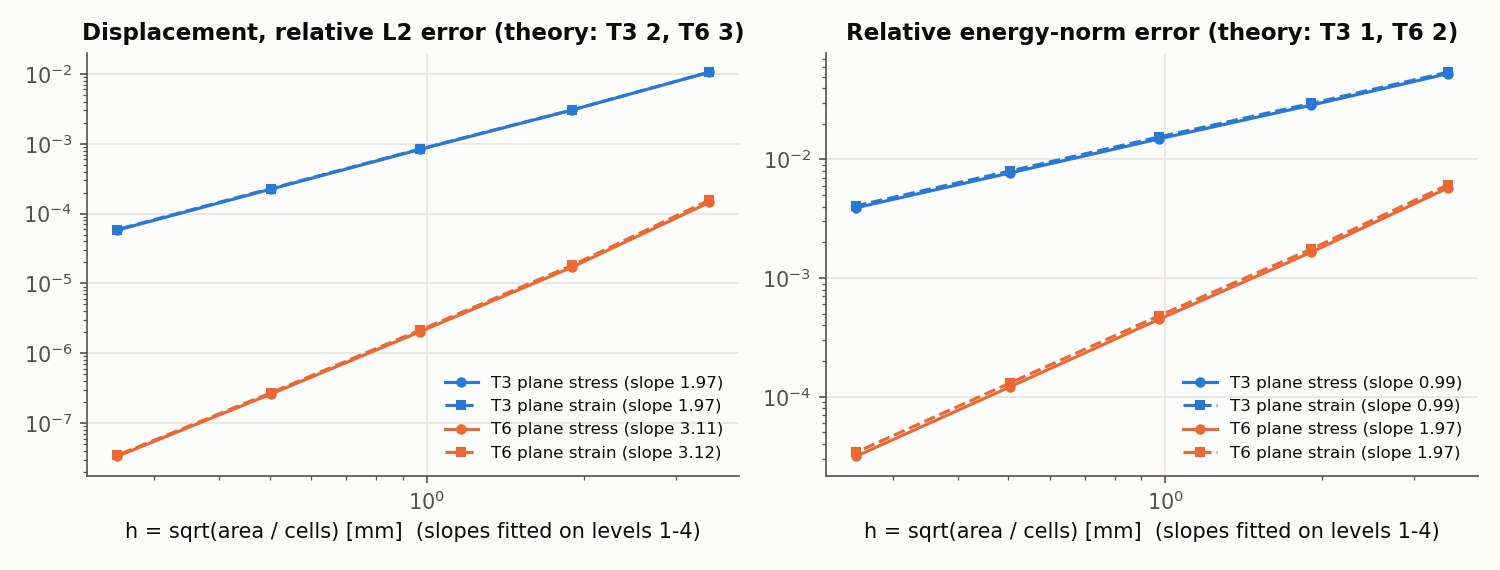
\includegraphics[width=\linewidth]{phase2_convergence}\caption{Kirsch plate (P2-f)}\end{subfigure}\hfill
  \begin{subfigure}{0.32\linewidth}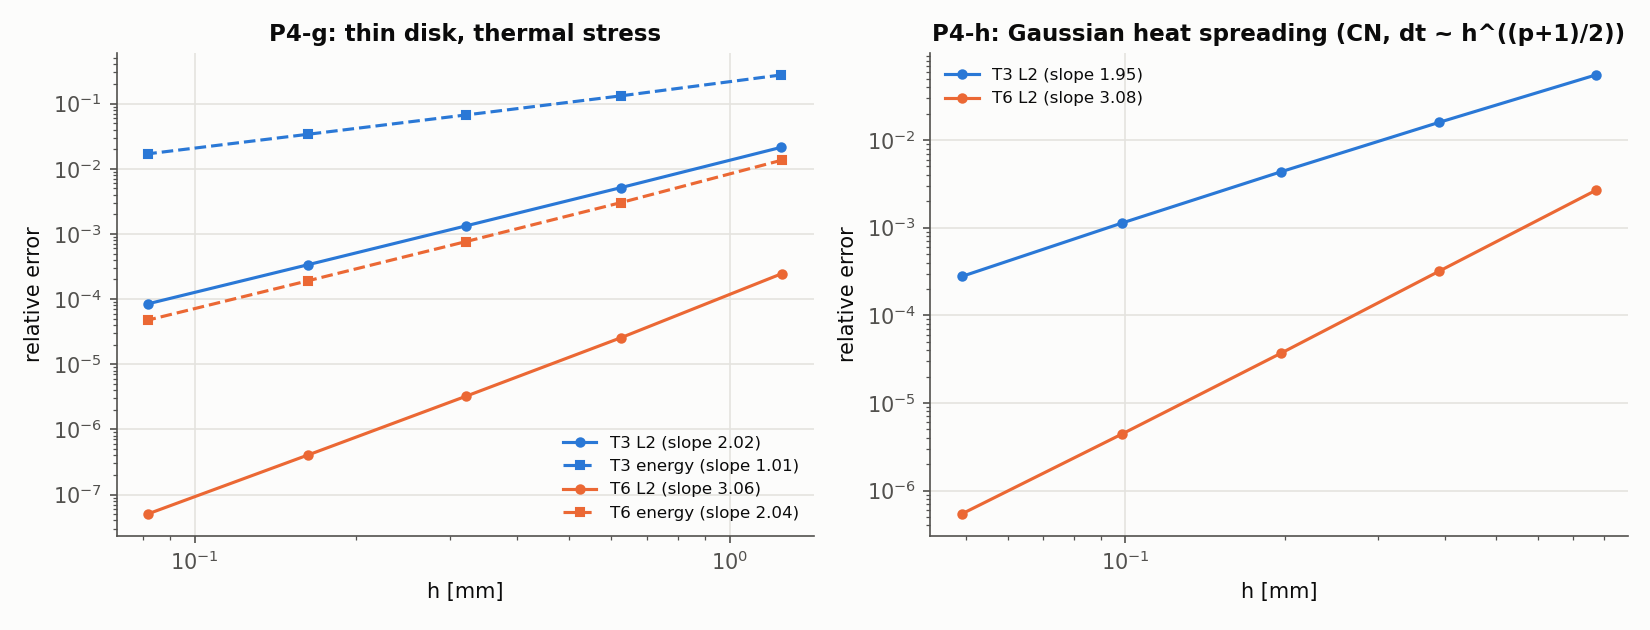
\includegraphics[width=\linewidth]{phase4_convergence}\caption{Thin disk, Gaussian (P4-g, h)}\end{subfigure}
  \caption{Observed convergence. Each claimed order is asserted within $\pm 0.15$ on levels 1--4.}
  \label{fig:conv}
\end{figure}

\begin{figure}[tbp]
  \centering
  \begin{subfigure}{0.49\linewidth}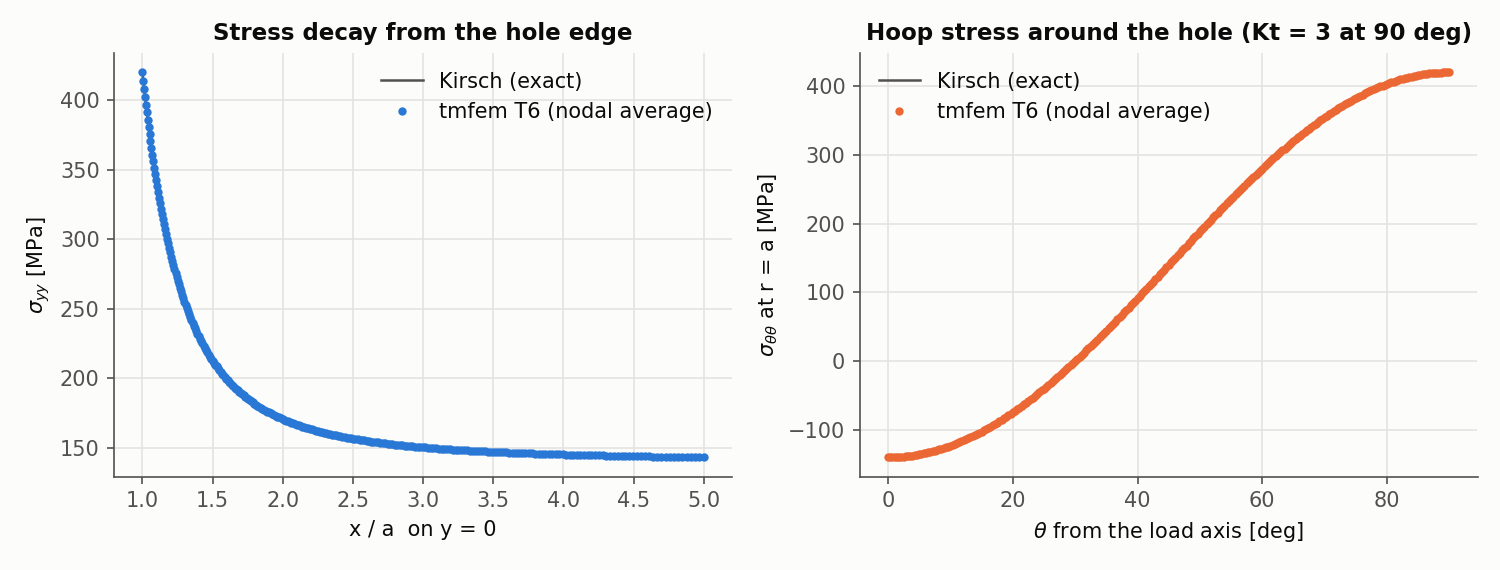
\includegraphics[width=\linewidth]{phase2_kirsch_profiles}\caption{Kirsch: FE against exact stresses}\end{subfigure}\hfill
  \begin{subfigure}{0.49\linewidth}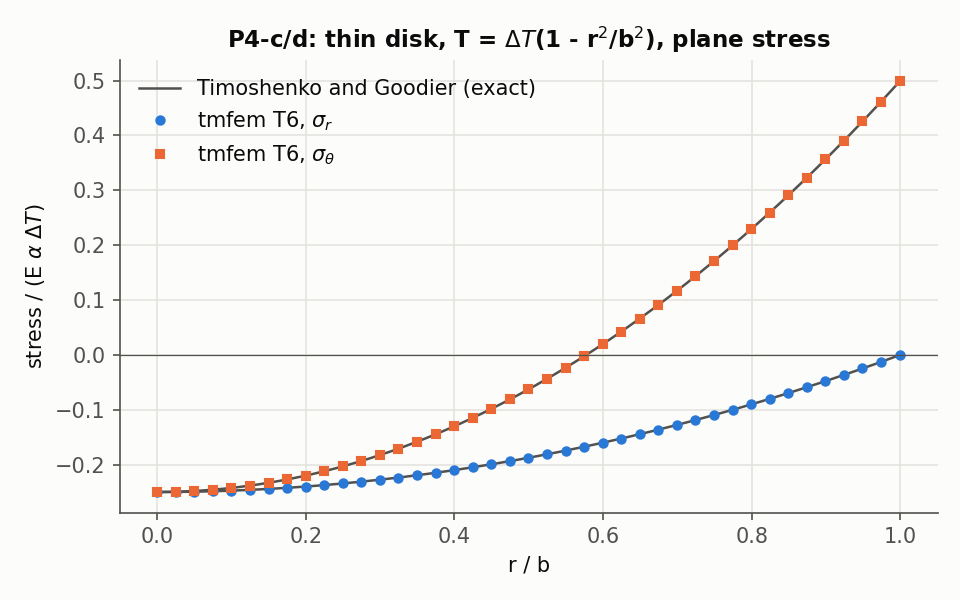
\includegraphics[width=\linewidth]{phase4_thin_disk}\caption{Thin disk: FE against Timoshenko--Goodier}\end{subfigure}
  \caption{Point stresses against closed-form solutions (T6, finest mesh).}
  \label{fig:profiles}
\end{figure}

\subsection{Elastoplasticity}\label{sec:plasticity}
\emph{Parameter identification} (\refrow{P3-a}, \cref{fig:plastic}a). With $\sigma_{y}$ fixed at the
yield point, a log-log fit reproduces the recomputed reference ($m = \NLogLogM$, $K = \NLogLogK~\si{MPa}$).
The deliverable is a three-parameter least-squares fit on stress: $\sigma_{y0} = \NFitSy~\si{MPa}$,
$K = \NFitK~\si{MPa}$, $m = \NFitM$, with residual standard deviation \NFitS~\si{MPa}. The source
gives 310.86~MPa, 559.27~MPa and 0.4077. The jackknife standard errors are much larger than the
covariance ones, because no data lie between $\alpha = 0$ (the yield point) and $\alpha = \NAlphaGap$, so
the yield point alone fixes the knee. This is a limit of the eight-point data set, not of the solver.

\emph{Material point} (\refrow{P3-b}). With tabulated hardening at $\sigma = \SI{457.24}{MPa}$ the
uniaxial driver gives $\varepsilon_{yy} = \NPbEyy$ and $\varepsilon_{xx} = \varepsilon_{zz} = \NPbExx$,
against the Abaqus values 0.03158 and $-0.01535$. The check is nearly tautological for
$\varepsilon_{yy}$, since 457.24~MPa is a data point. The lateral strain is the informative part:
$-\nu\sigma/E$ elastic plus $-\alpha/2$ plastic. With Ludwik hardening (\refrow{P3-c}) the driver
follows the data within \NPcZ{} residual standard deviations. This band is a weak test: with eight
points and three parameters no residual can exceed $\sqrt{\NFitDof}\,s = \NBandMax\,s$.

\emph{Newton convergence} (\refrow{P3-d}). The observed rate in the last iterations of a load step is
\NPdRatePe{} (plane strain) and \NPdRatePs{} (plane stress) on the uniform FE bar with Ludwik hardening.
This shows that the tangent is consistent along the loading path. The full global tangent is
also compared with central differences of the internal force on a non-uniform plastic Kirsch state.
\emph{FE bar against the driver} (\refrow{P3-e}): a uniform plane-strain bar meshed with T3 or T6
reproduces the material point with $\varepsilon_{zz} = 0$ to \NPeBar{} relative at every load step.

\emph{Hole plate at $S = \SI{140}{MPa}$} (\refrow{P3-f}, report only, \cref{fig:plastic}b). The elastic
peak of 420~MPa exceeds the yield stress, so a plastic zone forms. In plane stress, the thin plate of the
source's Abaqus model, the T6 level-4 solution gives an edge strain $\varepsilon_{yy} = \NPsEpsFE$, a
peak equivalent plastic strain of \NPsAlphaFE{} and $\sigma_{yy} = \NPsSigFE~\si{MPa}$ at the quadrature
point nearest the edge. The plastic zone extends \NPsZone{}$\,a$ from the hole. Neuber's rule
$\sigma\varepsilon = (K_t S)^2/E$~\cite{neuber1961}, solved on the same hardening curve, gives
$\varepsilon = \NNeuberEps$, $\alpha = \NNeuberAlpha$ and $\sigma = \NNeuberSig~\si{MPa}$. The FE strain
differs by \NPsEpsDiff{} and the plastic strain by \NPsAlphaDiff{}, while the stresses differ by
\NPsSigDiff{}. Neuber usually overestimates notch strains, and it is reported as an estimate, not a
target. In plane strain the notch root is biaxial ($\sigma_{zz} = \NPeSzz~\si{MPa}$ near the edge), and
the uniaxial rule does not apply.

\begin{figure}[tbp]
  \centering
  \begin{subfigure}{0.49\linewidth}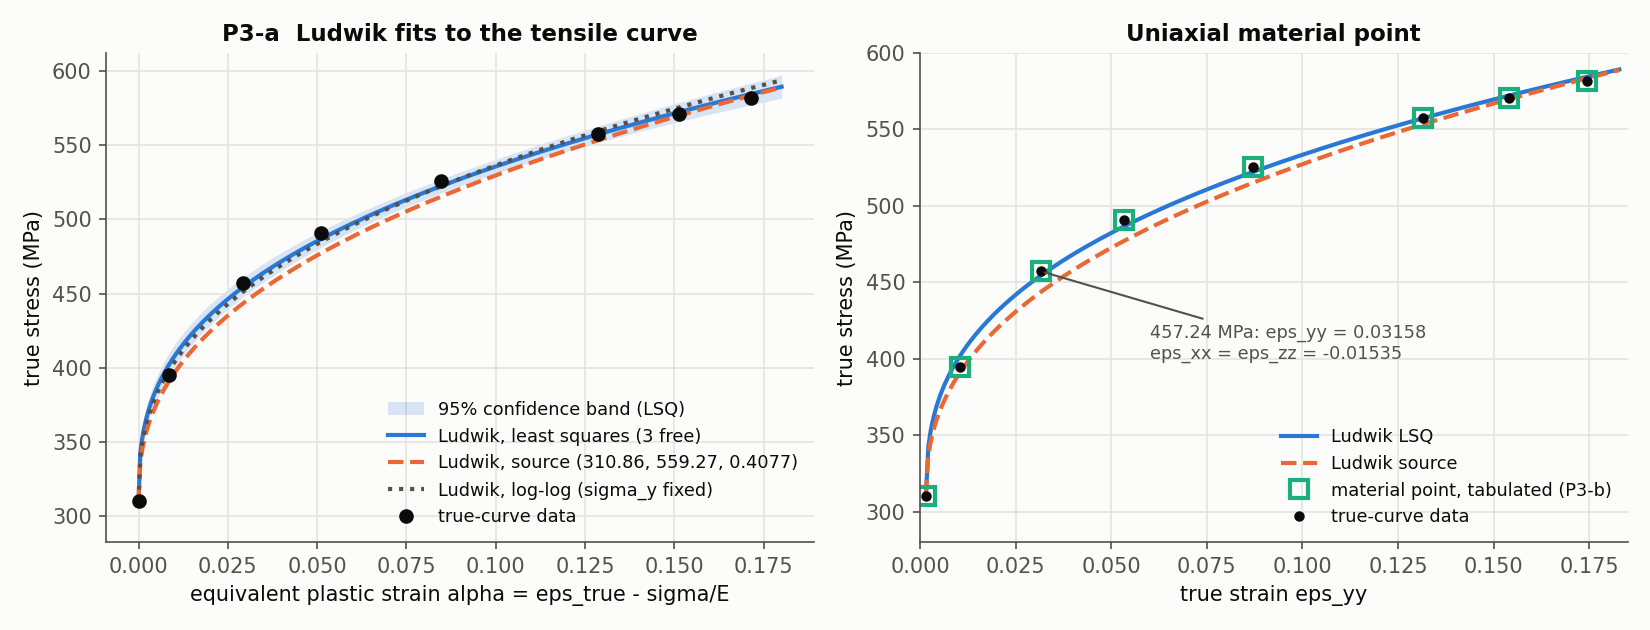
\includegraphics[width=\linewidth]{phase3_tensile_fit}\caption{Tensile data, fits and material point}\end{subfigure}\hfill
  \begin{subfigure}{0.49\linewidth}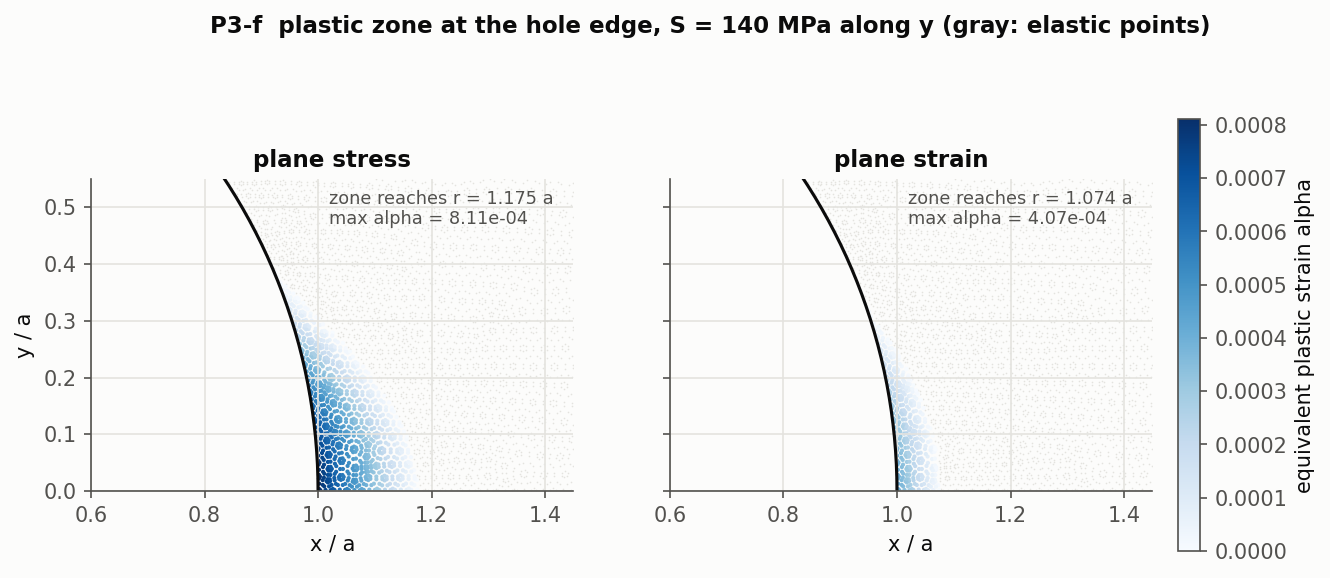
\includegraphics[width=\linewidth]{phase3_plastic_zone}\caption{Plastic zone at the hole, $S = 140$~MPa}\end{subfigure}
  \caption{Elastoplasticity: parameter identification and the hole plate.}
  \label{fig:plastic}
\end{figure}

\subsection{Thermo-mechanical coupling and 2D heat}
A bar held in $x$ under a uniform temperature rise (\refrow{P4-a}) and a free body (\refrow{P4-b}) are
reproduced to round-off in both plane states. They check $\beta$, the thermal load and stress recovery,
including $\sigma_{zz}$ in plane strain. For a thin disk with $T = \Delta T(1 - r^2/b^2)$
(\refrow{P4-c}, \refrow{P4-d}, \cref{fig:profiles}b) the Timoshenko--Goodier solution~\cite{timoshenko_goodier}
gives $\sigma_r/(E\alpha\Delta T) = -0.25$, $-0.1875$, $0$ at $r/b = 0$, $0.5$, $1$. The finest T6 mesh
gives \NDiskSrZero{}, \NDiskSrHalf{} and \NDiskSrOne{}, and for $\sigma_\theta$ it gives \NDiskStZero{},
\NDiskStHalf{}, \NDiskStOne{} (exact $-0.25$, $-0.0625$, $0.5$). The disk converges at orders
\NPgTthreeLtwo{} and \NPgTthreeEn{} (T3) and \NPgTsixLtwo{} and \NPgTsixEn{} (T6).

In 2D heat, an initial Gaussian spreading in a large domain (\refrow{P4-e}) keeps its variance on
$s_0^2 + 2\alpha t$ within \NGaussVarTthree{} (T3) relative, and it conserves energy to \NGaussEnTsix{}.
On straight T6 the variance identity holds almost by construction, so the $L^2$ error of the whole
profile is the real accuracy test (\refrow{P4-h}). It converges at order \NPhTthree{} (T3) and
\NPhTsix{} (T6). These are combined space--time orders along $\Delta t \propto h^{(p+1)/2}$ with CN; at
level~2 the time part is \NPhTimePartTthree{} (T3) and \NPhTimePartTsix{} (T6) of the error. The
source and convection terms (\refrow{P4-f}) pass three exactness checks: a steady slab with a uniform
source and Robin faces, a uniform plate cooled through its faces against the discrete amplification
factor, and a discrete energy balance. The last is an identity of the $\theta$-scheme, so the same test
also checks $\vect A\,(T_\infty\vect 1) = \vect F$ on a curved Robin rim with a face sink
(\NPfLoadIdentity{}), which a wrong load would fail.

\subsection{Errors found in the source, and disclosed changes}\label{sec:corrections}
\Cref{tab:corrections} lists the source values that the recomputation does not confirm. The test
targets are the recomputed values.

\begin{table}[tbp]
  \centering\footnotesize
  \begin{tabular}{@{}l p{3.3cm} p{3.4cm} p{3.4cm} p{3.0cm}@{}}
    \toprule
    Row & Quantity & Source says & Recomputed & Cause \\
    \midrule
    P1-a & steady flux $J$ & \SI{2.4e-12}{kg/(m^2.s)} & \SI{2.4e-9}{kg/(m^2.s)} & mm not converted \\
    P1-b & time to 0.8~wt\% & 7.025~h & 7.047~h & erf table interpolation \\
    P1-f & surface concentration & \SI{2.8e19}{cm^{-3}} & \SI{6.97e19}{cm^{-3}} & value matches $t = 36$~min \\
    P1-d & $D(\SI{1000}{K})$, $D(\SI{800}{K})$ & \SI{2.04e-13}{m^2/s}, \SI{2.11e-15}{m^2/s} & \SI{2.067e-13}{m^2/s}, \SI{2.140e-15}{m^2/s} & not identified \\
    P1-g & $D_0$, $D(\SI{1300}{\celsius})$ & \SI{3.2}{m^2/s}, \SI{5.86e-11}{m^2/s} & \SI{3.11}{cm^2/s}, \SI{1.74e-11}{cm^2/s} & unit slip ($D_0$); $D(\SI{1300}{\celsius})$ not identified \\
    P1-k & through-thickness $\Delta T$ & $<\SI{0.01}{K}$ & \SI{0.0255}{K} & infeasible for a 48~K swing \\
    P2-e & $\sigma_{rr}$ at $r = 1.5a$, $\theta = 0$ & 2100~MPa & 25.93~MPa & wrong table entry \\
    P3-a & Ludwik $m$, $K$ & 0.4077, 559.27~MPa & 0.385, 548~MPa & different point choice \\
    \bottomrule
  \end{tabular}
  \caption{Source values not confirmed by recomputation (\texttt{references/verify\_reference\_values.py}).}
  \label{tab:corrections}
\end{table}

Five changes to the test plan were made after a first run missed its target. Each was approved before
it was made, and \texttt{docs/VALIDATION.md} records the numbers from before the change.
(i)~\refrow{P1-k}: the original bound is physically infeasible and was replaced by the quasi-steady bound.
(ii)~\refrow{P2-f}: the T6 $L^2$ slope over levels 0--3 was outside $3 \pm 0.15$. The pairwise orders
were falling toward 3, so level~0 is pre-asymptotic. A finer level~4 was added, and the fit now uses
levels 1--4. The pass depends on dropping level~0, and this is stated.
(iii)~\refrow{P3-d}: on the Kirsch plate Newton reached round-off too fast for the pre-fixed rate
criterion, so the rate is asserted on the bar, where the active set is fixed by construction.
(iv)~\refrow{P4-e}: the variance test moved to the finest mesh after a constant $O(h^2)$
interpolation offset missed 0.5\% on level~2.
(v)~\refrow{P4-f}(iii): the plate is posed in excess temperature with $k = \SI{0.4}{W/(m.K)}$ instead of 400
(the target $G^n$ does not depend on $k$), because cancellation and a conduction-dominated solve at
$T_\infty = \SI{300}{K}$ exceeded $10^{-10}$ in floating point.
In addition, the \refrow{P4-c} tolerance was clarified in phase 4 to an absolute 0.0025 where the target is
zero ($\sigma_r$ at $r = b$). The CI runner is pinned to Ubuntu 24.04, not ``latest'', because the build requires Gmsh 4.12.1.

% ---------------------------------------------------------------------------------------------------
\section{Demonstration: a beam-heated block}\label{sec:demo}

\emph{This section is a demonstration, not a validation.} A Gaussian beam of rms size $s$ deposits
$E_l = \SI{1}{kJ}$ per metre of path in a pulse of \SI{10}{\micro s} into a long block of
$40\times40$~mm cross-section. The deposit is $q = E_l/(2\pi s^2\tau)\exp(-r^2/2s^2)$, a stand-in for
a FLUKA or Geant4 energy map, which would vary along the beam and would not be Gaussian. The pulse is
adiabatic, and afterwards the outer edges cool by convection ($h = \SI{10}{W/(m^2.K)}$). The
cross-section is solved in plane strain on T6 meshes refined to $s/10$ near the axis, for
$s = 0.5$, 1, 2 and \SI{4}{mm}. A long free block is really in generalised plane strain. The
difference is a uniform $\sigma_{zz}$ shift of \NDemoCuHalfgps{} to \NDemoCuFourgps{} of the peak
$\lvert\sigma_{zz}\rvert$ for copper (graphite: up to \NDemoGrFourgps{}), and twice that fraction in the
centre von Mises stress. The materials are annealed OFE copper~\cite{cda_c10100,ledbetter_naimon1974}
and isotropic graphite (SGL R4550~\cite{sgl_r4550}, with $\nu = 0.2$ and $c$ from NIST-JANAF~\cite{janaf}
assumed, because the data sheet does not give them). Every property and its source is recorded in
\texttt{cases/beam\_block/README.md}.

\begin{figure}[tbp]
  \centering
  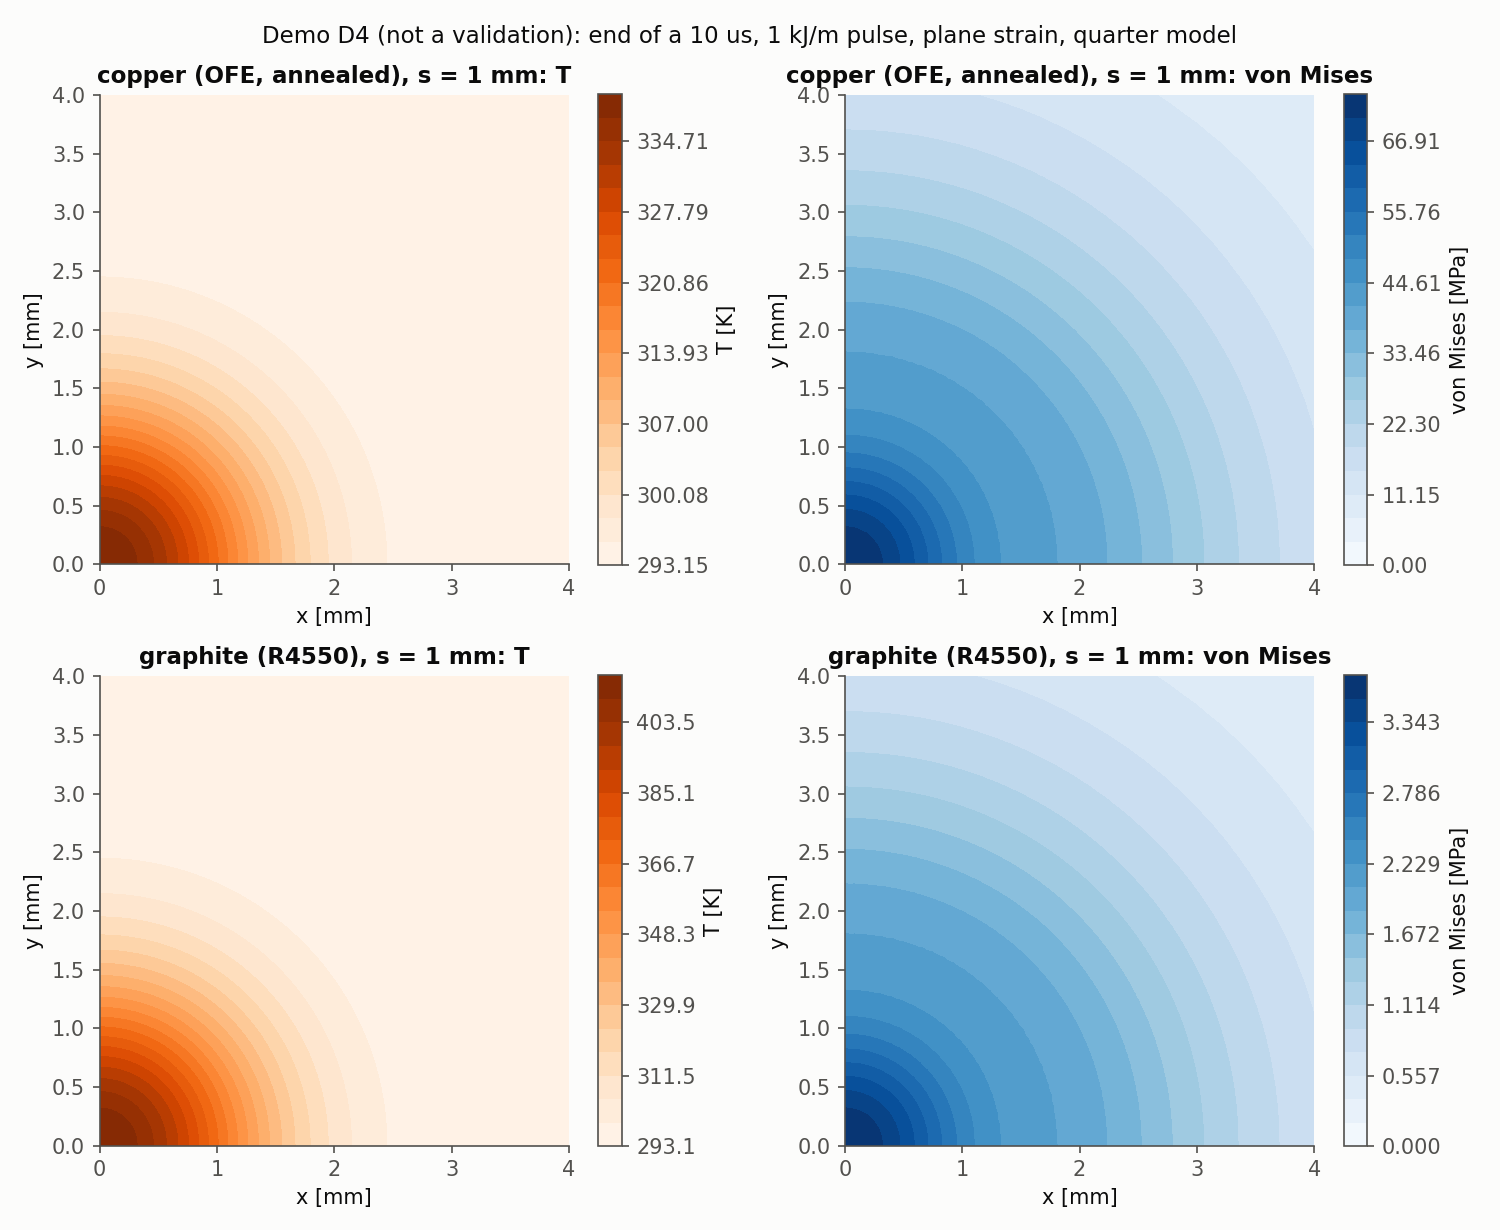
\includegraphics[width=\linewidth]{phase4_beam_block_maps}\\[0.5em]
  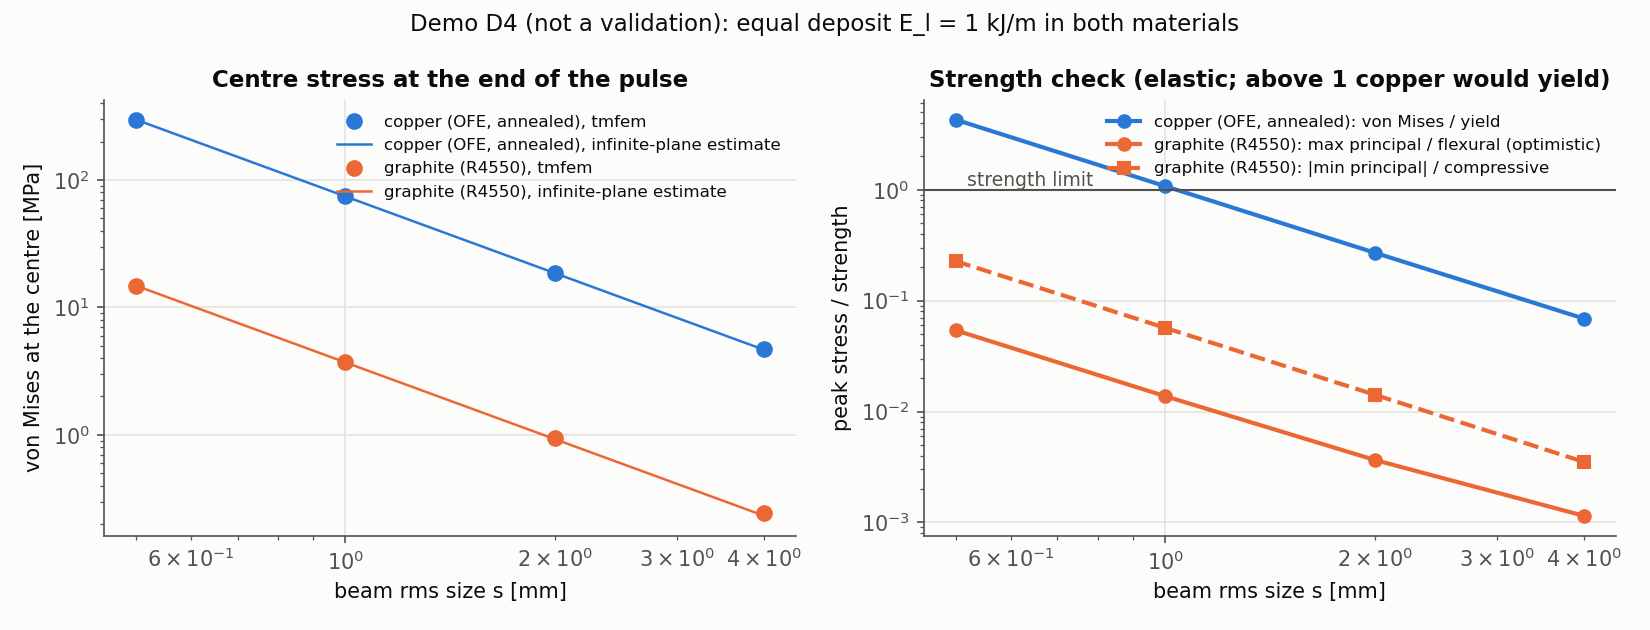
\includegraphics[width=0.72\linewidth]{phase4_beam_block_sweep}
  \caption{Demo D4 (not a validation). Top: temperature and von Mises stress at the end of the pulse.
  Bottom: centre stress and strength ratios against beam size.}
  \label{fig:demo}
\end{figure}

\paragraph{Results (\cref{fig:demo}).} The FE centre values agree with closed-form infinite-plane
estimates within \NDemoGapdT{} (temperature, which diffuses during the pulse) and \NDemoGapvm{} (von
Mises, because the section is finite). At $s = \SI{1}{mm}$ copper heats by \NDemoCuOnedT~\si{K} and
carries \NDemoCuOnevm~\si{MPa} von Mises at the centre, while graphite heats by \NDemoGrOnedT~\si{K}
and carries only \NDemoGrOnevm~\si{MPa}. Graphite's temperature rise is larger because its $\rho c$ is \NHeatRatio{} times lower. It is less stressed because the stress scales with the thermal-shock figure of merit
$E\alpha/((1-\nu)\rho c)$, which is \NFomGr~\si{Pa.m^3/J} for graphite against \NFomCu~\si{Pa.m^3/J}
for copper. The stress is mostly compressive and out of plane: the cold surroundings prevent the hot
core from expanding. The peak stress falls as $1/s^2$. Annealed copper (yield \NCuYield~\si{MPa})
exceeds yield for $s \le \SI{1}{mm}$: the ratio of von Mises stress to yield is \NDemoCuHalfratio{}
at \SI{0.5}{mm} and \NDemoCuOneratio{} at \SI{1}{mm}. Graphite reaches only \NDemoGrHalfratio{} of its
flexural strength and \NDemoGrHalfcomp{} of its compressive strength, even at \SI{0.5}{mm}. The tensile
check is optimistic, because flexural strength overestimates tensile strength. This illustrates one reason
graphite is used in dumps and absorbers, its thermal-shock resistance. Its other main advantage, a lower
energy density for the same beam thanks to its low density and atomic number, is outside this demo,
which fixes the deposited energy. After the pulse the stresses relax as
heat diffuses over the spot: for copper at $s = \SI{1}{mm}$ the centre stress is \NRelaxTenms{} of its
peak at \SI{10}{ms} and \NRelaxHundredms{} at \SI{100}{ms}, long before convection removes the energy.

\paragraph{Validity.} The results are elastic with constant properties. Above yield, copper would need
thermoplasticity. With constant $c$, graphite at $s = \SI{0.5}{mm}$ reaches \NDemoGrHalfTmax~\si{K}, but
its specific heat at \SI{800}{K} is \NCpRatio{} times the room-temperature value. Integrating the JANAF
$c(T)$ for the same deposit gives a rise of \NJanafdT~\si{K} (to \NJanafT~\si{K}) instead of
\NConstdT~\si{K}, so that row overestimates the temperature rise by \NJanafOver{}.

% ---------------------------------------------------------------------------------------------------
\section{Limitations}\label{sec:limitations}
\begin{itemize}\setlength\itemsep{1pt}
  \item \textbf{Out of scope by design:} 3D, large deformation, dynamics and stress waves,
  temperature-dependent properties, contact, radiation, real energy maps. A \SI{10}{\micro s} pulse is
  long compared with the acoustic transit time of a millimetre spot, but stress waves are not modelled.
  \item \textbf{Elements and materials:} triangles only (T3, T6); one isotropic material per run; unit
  thickness; no body force. J2 plasticity with isotropic hardening only, so there is no Bauschinger
  effect. The model is rate-independent and isothermal. The tabulated law has slope jumps, so quadratic
  Newton convergence is asserted with Ludwik hardening only.
  \item \textbf{Benchmarks:} the Kirsch plate uses infinite-plate tractions, not the finite plate of the
  source's Abaqus model. The elastoplastic hole plate keeps elastic Kirsch tractions on its outer
  boundary, which is an approximation once a plastic zone exists, and is reported only. The steel-plate
  case is validated against a lumped model with a synthetic input, not against ANSYS (\refrow{P1-l}
  is skipped). The fit uncertainty describes eight digitised points and model misfit, not material
  scatter.
  \item \textbf{Time integration:} fixed time steps without error control. In 2D only consistent
  capacity is available, because row-sum lumping gives zero capacity to T6 corner nodes.
  \item \textbf{Reproducibility:} meshes come from Gmsh 4.12.1. Another version would give slightly
  different meshes and numbers, so the build refuses other versions.
  \item \textbf{Demo:} plane strain instead of generalised plane strain, Gaussian deposit, elastic
  constant-property analysis, and assumed graphite $\nu$ and $c$ (\cref{sec:demo}).
\end{itemize}

% ---------------------------------------------------------------------------------------------------
\section{Conclusion and outlook}\label{sec:conclusion}
\tmfem{} implements, from scratch, the chain of methods behind a thermal-stress analysis of a
beam-heated component. Each link is tied to a test against an independent answer, including observed
convergence orders for every discretisation. The process found several errors in the reference
material, and every deviation from the original test plan is disclosed. Possible next steps, not
attempted here, are stress-intensity factors by the domain $J$-integral for a cracked strip, OpenMP
assembly, temperature-dependent properties with thermoplasticity for the demo, and generalised plane
strain.

\paragraph{Credits.} Benchmark cases adapted from M.~R.~Kabiri, ENSAM Mekn\`es lab
materials~\cite{kabiri_labs}, with permission. Analytical solutions from the cited textbooks.

\bibliographystyle{unsrtnat}
\bibliography{refs}

\appendix
\section{Reproducing the numbers}\label{app:repro}
Requirements: a C++17 compiler, CMake $\ge$ 3.16, Eigen~3 and Gmsh 4.12.1 (Ubuntu 24.04:
\texttt{apt install libeigen3-dev gmsh}). Catch2 and nlohmann/json are fetched at pinned versions.
\begin{verbatim}
cmake -S . -B build -DCMAKE_BUILD_TYPE=Release
cmake --build build -j
ctest --test-dir build -V > results/ctest_full.log 2>&1
./build/src/tmfem cases/beam_block/copper.json    # demo, section 4
./build/src/tmfem cases/beam_block/graphite.json
python3 scripts/build_results_table.py            # README table
python3 scripts/report_numbers.py                 # numbers, provenance
cd report && latexmk -pdf main.tex
\end{verbatim}
\texttt{docs/PROVENANCE.md} lists every macro used in this report with its value, source file and
the test or command that produced it.

\end{document}
